\documentclass[11pt,a4paper]{article}

\usepackage[T1]{fontenc}
\usepackage[utf8]{inputenc}
\usepackage[italian]{babel}
\usepackage{amsmath,amssymb}
\usepackage[a4paper,margin=2.5cm]{geometry}
\usepackage{array}
\usepackage{siunitx}
\usepackage{booktabs}
\usepackage{graphicx}
\usepackage{float}
\usepackage{hyperref}

\hypersetup{hidelinks}
\setlength{\parindent}{0pt}
\setlength{\parskip}{4pt}
\allowdisplaybreaks
\graphicspath{{figure/}}
\sisetup{output-decimal-marker={,}, group-separator={\,}, per-mode=symbol,
         exponent-product=\cdot, range-phrase={\text{--}}}

\newcommand{\Ru}{R_1}
\newcommand{\Rd}{R_2}
\newcommand{\uma}{u-a}
\newcommand{\upa}{u+a}
\newcommand{\Cr}{C}

\title{Gasdinamica -- Svolgimento esercizio 3\\[2pt]
\large Condizione al contorno d'ingresso a temperatura totale costante: derivate nel tempo di pressione e velocità}
\author{}
\date{Prova del 01/01/1975}

\begin{document}
\maketitle

\section*{Traccia}
Determinare le derivate nel tempo della pressione e della velocità al contorno di ingresso di un flusso
monodimensionale, non stazionario, subsonico e omoentropico con condizione assegnata di temperatura totale costante.
\begin{figure}[H]
  \centering
  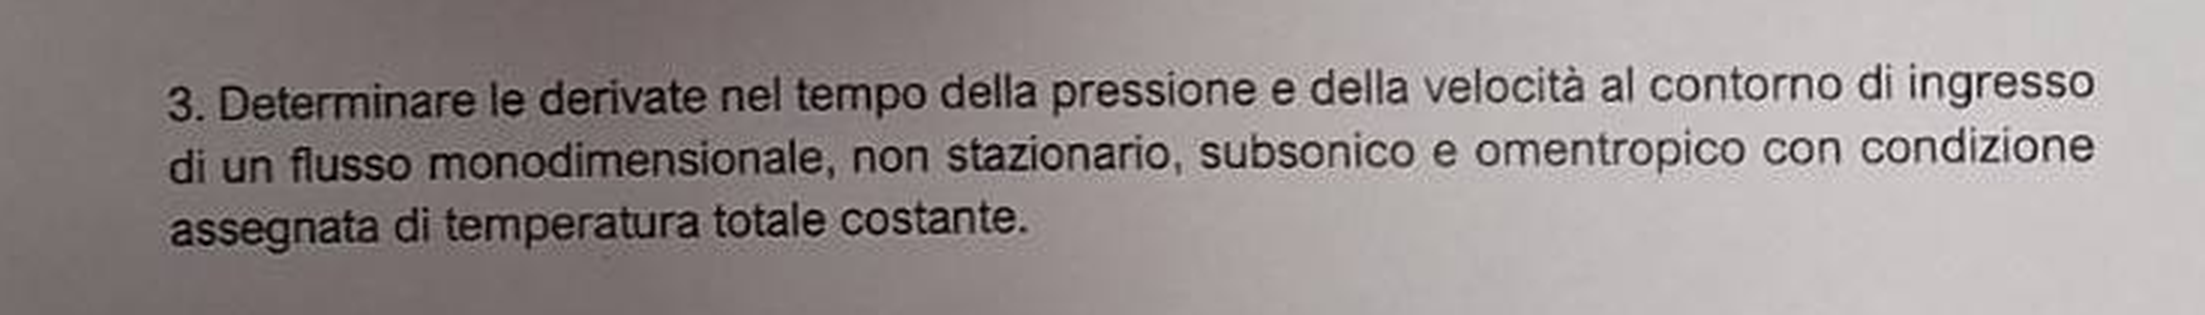
\includegraphics[width=0.85\textwidth]{originale.png}
  \caption{Testo originale dell'esercizio.}
\end{figure}
Tracce affini nel catalogo: B68-E02 (04/02/2022), ingresso con portata ed entalpia totale costanti; B53-E02
(17/02/2017), ingresso con $\rho u$ e $T$ costanti; B53-E09, ammissibilità di un contorno con $T_0$, $s$ e $\rho u$
costanti; per l'uscita, B70-E02 (13/02/2023), Mach imposto.

%==============================================================================
\section{Lettura del testo e dati}
\begin{itemize}
  \item \textbf{Contorno d'ingresso}: il gas entra nel condotto. Pongo l'ingresso all'estremo sinistro, $x=0$, con
        il condotto per $x>0$; quindi $u>0$.
  \item \textbf{Subsonico}: $0<u<a$, cioè $0<M<1$ nella sezione d'ingresso.
  \item \textbf{Omoentropico}: $s$ uniforme nello spazio e costante nel tempo.
  \item \textbf{Temperatura totale costante}: $T_0=T+u^2/(2c_p)$ è assegnata e non varia nel tempo. Con
        $a^2=\gamma RT$ e $c_p=\gamma R/(\gamma-1)$ la condizione si scrive
        \[
          a^2+\delta u^2=a_0^2=\text{cost},\qquad \delta=\frac{\gamma-1}{2}.
        \]
  \item \textbf{Richiesta}: $p_t$ e $u_t$ nella sezione d'ingresso, cioè come evolvono pressione e velocità al
        contorno in funzione di ciò che arriva dall'interno.
\end{itemize}
Non ci sono dati numerici: svolgo il problema in forma letterale e uso un esempio per l'aria ($\gamma=1{,}4$,
$\delta=0{,}2$) solo per i diagrammi: $M_1=0{,}3$ all'ingresso, grandezze totali $p_0=a_0=1$, onda incidente con
$p_2/p_1=1{,}1$ (compressione) e $0{,}9$ (espansione).

%==============================================================================
\section{Modello e ipotesi}
\begin{itemize}
  \item \textbf{Eulero 1D instazionario}: gas perfetto, non viscoso, adiabatico, condotto a sezione costante con
        onde piane (lunghezze d'onda molto maggiori del diametro).
  \item \textbf{Omoentropico}, come dice il testo: $s_x=0$ e $s_t=0$, quindi $\rho_x=p_x/a^2$, $\rho_t=p_t/a^2$, e
        valgono gli invarianti di Riemann $\Ru=a-\delta u$ lungo le $\uma$ e $\Rd=a+\delta u$ lungo le $\upa$. Le onde
        restano continue (nessun urto).
  \item La condizione $T_0=\text{cost}$ vale \textbf{in ogni istante} nella sezione d'ingresso: ciò che la
        realizza a monte (un grande serbatoio o l'ambiente) risponde in modo quasi stazionario rispetto ai tempi
        delle onde nel condotto. $T_0$ è costante \textbf{solo nella sezione d'ingresso}, dove è imposta: nel
        condotto il flusso è instazionario e attraverso le onde $T_0$ e $p_0$ cambiano (nell'esempio, dietro la
        compressione incidente, $T_0$ cresce del 2\,\% e $p_0$ del 7\,\%).
  \item Le derivate spaziali nella sezione d'ingresso sono quelle \textbf{dal lato del condotto}: solo la
        perturbazione che esce dal dominio è nota dall'interno.
\end{itemize}

%==============================================================================
\section{Analisi qualitativa}
\textbf{Quante condizioni.} Nella sezione d'ingresso, con $0<u<a$, le caratteristiche $\upa$ e $u$ hanno pendenza
positiva ed \textbf{entrano} nel condotto, mentre la $\uma$ ($u-a<0$) arriva dall'interno ed \textbf{esce}. Servono
quindi \textbf{due} condizioni. La traccia ne dà due: l'omoentropia fissa l'entropia del gas che entra (onda di
entropia, famiglia $u$), $T_0$ costante fornisce la seconda. Il problema è ben posto: non c'è sovraspecificazione e
la variabile d'onda uscente, portata dalla $\uma$, non è prescritta ma viene dall'interno.

\textbf{Le due condizioni equivalgono a un serbatoio.} Con $s$ costante, $p/T^{\gamma/(\gamma-1)}$ è costante; poiché
$p_0=p\,(T_0/T)^{\gamma/(\gamma-1)}$, anche $p_0$ è costante. Imporre $s$ e $T_0$ equivale quindi a imporre $p_0$ e
$T_0$: è l'ingresso da un grande serbatoio, in cui non si impone la pressione statica.

\textbf{Che cosa mi aspetto.} Nella sezione d'ingresso $h_0$ e $s$ sono costanti, quindi pressione e velocità sono
legate come in Bernoulli: se la velocità cala, la pressione sale, ma di poco quando $M$ è piccolo. A basso Mach
l'ingresso si comporta quasi come un estremo a pressione imposta. Un'onda $\uma$ che arriva dall'interno si riflette
come onda $\upa$ di \textbf{natura opposta}, con ampiezza minore di quella dell'incidente. Avvicinandosi a $M=1$ la
caratteristica uscente diventa verticale e l'ingresso tende a strozzarsi.

%==============================================================================
\section{Topologia del campo}
Nel piano $x$--$t$ vicino all'ingresso (fig.~\ref{fig:xt}) ci sono queste regioni:
\begin{itemize}
  \item \textbf{1}: flusso iniziale uniforme, subsonico, con $a_1^2+\delta u_1^2=a_0^2$;
  \item \textbf{onda incidente $\uma$}: onda semplice che arriva dall'interno, a $\Rd$ uniforme;
  \item \textbf{2}: stato uniforme dietro l'incidente, a $R_{2,2}=R_{2,1}$;
  \item \textbf{Z}: zona d'interazione a due famiglie a ridosso dell'ingresso, fra l'arrivo della testa e quello
        della coda dell'incidente, chiusa dal punto P;
  \item \textbf{onda riflessa $\upa$}: onda semplice a $\Ru$ uniforme, che scende il condotto nello stato 2;
  \item \textbf{3}: stato uniforme all'ingresso dopo la riflessione, a $R_{1,3}=R_{1,2}$, che soddisfa la condizione.
\end{itemize}
Per gli stati uniformi tratto le caratteristiche come semirette. La zona Z non serve risolverla: le derivate che
ricavo valgono nella sezione d'ingresso istante per istante, anche mentre vi arriva l'onda.

%==============================================================================
\section{Bilancio equazioni/incognite}
Nella sezione d'ingresso le incognite sono le tre derivate nel tempo $p_t$, $u_t$, $\rho_t$ e le due variabili
d'onda entranti, quelle delle famiglie $\upa$ e $u$:
\[
  X=p_x+\rho a\,u_x \quad(\upa),\qquad Z=\rho_x-\frac{p_x}{a^2}\quad(u).
\]
La variabile d'onda uscente $Y=p_x-\rho a\,u_x$ ($\uma$) è nota dall'interno. Le incognite sono 5. Le equazioni di
Eulero in forma caratteristica sono 3, quindi servono \textbf{2} equazioni al contorno, da scrivere in forma
differenziale: l'omoentropia e $T_0$ costante. Il conteggio torna con quello delle caratteristiche entranti.

%==============================================================================
\section{Calcolo}
\subsection{Equazioni di Eulero nella sezione d'ingresso}
Parto dalle equazioni quasi lineari per $p$ e $u$, con $\gamma p=\rho a^2$:
\[
  p_t+u\,p_x+\rho a^2u_x=0,\qquad u_t+u\,u_x+\frac{p_x}{\rho}=0 .
\]
Moltiplico la seconda per $\rho a$ e la sommo o la sottraggo alla prima:
\[
  (p_t+\rho a\,u_t)+(u+a)\,X=0,\qquad (p_t-\rho a\,u_t)+(u-a)\,Y=0 .
\]
La prima è la compatibilità lungo la $\upa$, la seconda lungo la $\uma$. Risolvendo rispetto a $p_t$ e $u_t$ si
ottiene la forma con le onde separate:
\[
  p_t=-\frac{u+a}{2}X-\frac{u-a}{2}Y,\qquad u_t=-\frac{u+a}{2\rho a}X+\frac{u-a}{2\rho a}Y .
\]
L'entropia, $s_t+u\,s_x=0$, dà la terza equazione, $(\rho_t-p_t/a^2)+u\,Z=0$.

\subsection{Le condizioni al contorno in forma differenziale}
\textbf{Omoentropia.} $Z=0$ e $s_t=0$, quindi
\[
  \rho_t=\frac{p_t}{a^2}.
\]
L'equazione dell'entropia è soddisfatta identicamente: non entra alcuna onda di entropia.

\textbf{Temperatura totale costante.} Derivo $h_0=h+u^2/2$ nel tempo e uso Gibbs, $T\,ds=dh-dp/\rho$, con $ds=0$:
\[
  h_{0,t}=h_t+u\,u_t=\frac{p_t}{\rho}+u\,u_t=0\qquad\Longrightarrow\qquad p_t=-\rho u\,u_t .
\]
È Bernoulli scritto nel tempo nella sezione d'ingresso.

\subsection{Derivate di velocità e pressione}
Nella compatibilità lungo la $\uma$, $p_t-\rho a\,u_t=(a-u)\,Y$, sostituisco $p_t=-\rho u\,u_t$:
$-\rho(a+u)\,u_t=(a-u)\,Y$. Quindi
\[
  \boxed{\;u_t=-\frac{1}{\rho}\,\frac{1-M}{1+M}\,\bigl(p_x-\rho a\,u_x\bigr),\qquad
  p_t=u\,\frac{1-M}{1+M}\,\bigl(p_x-\rho a\,u_x\bigr)\;}
\]
con $M=u/a$ e $p_x-\rho a\,u_x$ calcolata dal lato del condotto. Ne seguono
\[
  \rho_t=\frac{p_t}{a^2},\qquad \frac{T_t}{T}=\frac{\gamma-1}{\gamma}\,\frac{p_t}{p},\qquad
  \frac{\dot m_t}{\dot m}=\frac{\rho_t}{\rho}+\frac{u_t}{u}=(1-M^2)\,\frac{u_t}{u},
\]
dove $\dot m=\rho u$ è la portata per unità di area. Le derivate dipendono solo dallo stato nella sezione e dalla
perturbazione uscente $Y$. Se dall'interno non arriva nulla ($Y=0$), lo stato all'ingresso non cambia.

\subsection{Onda entrante e riflessione}
Dalla compatibilità lungo la $\upa$, $X=-(p_t+\rho a\,u_t)/(u+a)$, e con i risultati precedenti:
\[
  X=\left(\frac{1-M}{1+M}\right)^2 Y .
\]
In un'onda semplice $\uma$ è costante $\Rd$, quindi $dp=-\rho a\,du$ e $Y=2p_{x,i}$. In un'onda $\upa$, invece,
$dp=\rho a\,du$ e $X=2p_{x,r}$. Allora
\[
  p_{x,r}=\left(\frac{1-M}{1+M}\right)^2 p_{x,i}.
\]
I gradienti hanno lo stesso segno. Un'incidente $\uma$ di compressione, che si muove verso l'ingresso, ha il gas
compresso dietro di sé, a destra: $p_{x,i}>0$. Allora $p_{x,r}>0$, e la riflessa $\upa$, che va verso destra, ha la
pressione più bassa dietro di sé: è un'\textbf{espansione}. Allo stesso modo un'espansione si riflette come
compressione.

Nel tempo, nella sezione d'ingresso, $p_{t,i}=(a-u)\,p_{x,i}$ e $p_{t,r}=-(a+u)\,p_{x,r}$, quindi
\[
  \boxed{\;\frac{\Delta p_r}{\Delta p_i}=\Cr=-\frac{1-M}{1+M}\;}
\]
per onde acustiche. Lo stesso coefficiente vale in modo esatto per gli invarianti: da $a\,da+\delta u\,du=0$,
$d\Ru=da-\delta\,du=-\delta(1+M)\,du$ e $d\Rd=da+\delta\,du=\delta(1-M)\,du$, cioè $d\Rd=\Cr\,d\Ru$. Nella sezione
d'ingresso le variazioni complessive sono
\[
  \Delta p=(1+\Cr)\,\Delta p_i=\frac{2M}{1+M}\,\Delta p_i,\qquad
  \Delta u=\frac{2}{1+M}\,\Delta u_i .
\]
Con $M$ da $0$ a $1$, $\Cr$ va da $-1$ a $0$ (tab.~\ref{tab:C}).

\begin{table}[H]
  \centering
  \begin{tabular}{ccccc}
    \toprule
    $M$ & $\Cr=\Delta p_r/\Delta p_i$ & $\Delta p/\Delta p_i=\frac{2M}{1+M}$ & $\Delta u/\Delta u_i=\frac{2}{1+M}$ &
    $p_{x,r}/p_{x,i}=\Cr^2$ \\
    \midrule
    0,1 & $-0{,}818$ & 0,182 & 1,82 & 0,669 \\
    0,2 & $-0{,}667$ & 0,333 & 1,67 & 0,444 \\
    0,3 & $-0{,}538$ & 0,462 & 1,54 & 0,290 \\
    0,5 & $-0{,}333$ & 0,667 & 1,33 & 0,111 \\
    0,7 & $-0{,}176$ & 0,824 & 1,18 & 0,031 \\
    0,9 & $-0{,}053$ & 0,947 & 1,05 & 0,003 \\
    \bottomrule
  \end{tabular}
  \caption{Riflessione all'ingresso per l'aria in funzione del Mach d'ingresso.}
  \label{tab:C}
\end{table}

\subsection{Esempio numerico}
Per i diagrammi prendo $p_0=a_0=1$ e $M_1=0{,}3$. Dalle isentropiche
\[
  a_1=\frac{a_0}{\sqrt{1+\delta M_1^2}}=0{,}991,\qquad u_1=M_1a_1=0{,}297,\qquad
  p_1=p_0\left(1+\delta M_1^2\right)^{-\gamma/(\gamma-1)}=0{,}940 .
\]
\textbf{Compressione incidente}, $p_2/p_1=1{,}1$. Attraverso la $\uma$ resta costante $\Rd$, quindi
\[
  a_2=a_1\left(\frac{p_2}{p_1}\right)^{(\gamma-1)/(2\gamma)}=1{,}005,\qquad u_2=u_1-\frac{a_2-a_1}{\delta}=0{,}229,
  \qquad p_2=1{,}033 .
\]
Lo stato 3 ha $a_3-\delta u_3=R_{1,2}$ (portato dalle $\uma$ attraverso la riflessa) e $a_3^2+\delta u_3^2=a_0^2$.
Sostituendo $a_3=R_{1,2}+\delta u_3$ nella seconda si ha un'equazione di secondo grado in $u_3$:
\[
  \delta(1+\delta)\,u_3^2+2\delta R_{1,2}\,u_3+R_{1,2}^2-a_0^2=0\;\Longrightarrow\;
  u_3=\frac{-\delta R_{1,2}+\sqrt{\delta(1+\delta)a_0^2-\delta R_{1,2}^2}}{\delta(1+\delta)} ,
\]
con la radice positiva perché il gas entra. Ottengo
\[
  u_3=0{,}188,\qquad a_3=0{,}997,\qquad M_3=0{,}189,\qquad p_3=p_0\left(\frac{a_3}{a_0}\right)^{2\gamma/(\gamma-1)}=0{,}975 .
\]
La riflessa porta la pressione da $1{,}033$ a $0{,}975$ ed è un'espansione, mentre la velocità scende ancora. La
portata cala: $\dot m_3/\dot m_1=0{,}65$. Per confronto, a pari onda incidente, un ingresso a pressione imposta
($p=p_1$) darebbe $u=0{,}162$ e un contorno a velocità imposta ($u=u_1$) darebbe $p=1{,}135$.

\textbf{Espansione incidente}, $p_2/p_1=0{,}9$. Con lo stesso procedimento
\[
  p_2=0{,}846,\quad u_2=0{,}371;\qquad p_3=0{,}889,\quad u_3=0{,}407,\quad M_3=0{,}413,\qquad
  \dot m_3/\dot m_1=1{,}31 .
\]
La riflessa è una compressione.

Con queste ampiezze il rapporto $\Delta\Rd/\Delta\Ru$ vale $-0{,}61$ per la compressione e $-0{,}47$ per
l'espansione, contro $\Cr(M_1)=-0{,}54$. La compressione abbassa il Mach all'ingresso e la riflessione si fa più
intensa; l'espansione lo alza e la riflessione si indebolisce.

%==============================================================================
\section{Verifiche a posteriori}
\begin{itemize}
  \item Numero di condizioni: due caratteristiche entranti ($\upa$, $u$) e due condizioni ($s$, $T_0$); la variabile
        uscente $Y$ non è prescritta: verificata.
  \item Stesso risultato con gli invarianti: da $a\,a_t+\delta u\,u_t=0$ e $(\Ru)_t=(a-u)(\Ru)_x$ si ottiene
        $u_t=-(a-u)(\Ru)_x/[\delta(1+M)]$, che coincide con la formula trovata perché
        $Y=(\rho a/\delta)(\Ru)_x$: verificata.
  \item Limite $M\to0$: $p_t\to0$ e $\Cr\to-1$, cioè l'estremo a pressione imposta: verificata.
  \item Limite $M\to1$: $u_t=p_t=0$ e $X=0$. La $\uma$ diventa verticale e lo stato resta quello critico,
        cioè l'ingresso sonico: verificata.
  \item Condizione nello stato 3 dell'esempio: $a_3^2+\delta u_3^2=a_0^2$ e $p_{0,3}=p_0$, in entrambi i casi:
        verificata.
  \item Ingresso ancora subsonico e in ingresso nell'esempio: $0<M_3<1$ ($0{,}189$ e $0{,}413$): verificata.
  \item Onda debole: con $p_2/p_1=1{,}0001$ il rapporto $\Delta\Rd/\Delta\Ru$ coincide con $\Cr(0{,}3)=-0{,}538$:
        verificata.
  \item Omoentropia: la riflessa di una compressione è un'espansione; quella di un'espansione è una compressione
        più debole e meno ripida ($p_{x,r}=\Cr^2p_{x,i}$), quindi l'urto non si forma vicino all'ingresso: verificata.
  \item Niente vuoto: $a_3^2=a_0^2-\delta u_3^2>0$ per ogni ingresso subsonico: verificata.
\end{itemize}

%==============================================================================
\section{Risultati}
\begin{table}[H]
  \centering
  \small
  \begin{tabular}{lll}
    \toprule
    Grandezza & Risultato & Esatto/approssimato \\
    \midrule
    condizioni al contorno & $s$ e $T_0$ costanti, equivalenti a $p_0$, $T_0$ & esatto \\
    legame al contorno & $p_t=-\rho u\,u_t$, $\rho_t=p_t/a^2$ & esatto \\
    derivata della velocità & $u_t=-\frac{1}{\rho}\frac{1-M}{1+M}(p_x-\rho a\,u_x)$ & esatto \\
    derivata della pressione & $p_t=u\,\frac{1-M}{1+M}(p_x-\rho a\,u_x)$ & esatto \\
    onda entrante & $p_x+\rho a\,u_x=\left(\frac{1-M}{1+M}\right)^2(p_x-\rho a\,u_x)$ & esatto \\
    onda riflessa & $\upa$, \textbf{natura opposta} all'incidente & esatto \\
    ampiezza & $d\Rd=-\frac{1-M}{1+M}d\Ru$; $\Delta p_r\approx\Cr\Delta p_i$ & esatto; acustico \\
    portata & $\dot m_t/\dot m=(1-M^2)\,u_t/u$ & esatto \\
    \bottomrule
  \end{tabular}
  \caption{Risultati.}
\end{table}

%==============================================================================
\section{Rappresentazioni}
\begin{figure}[H]
  \centering
  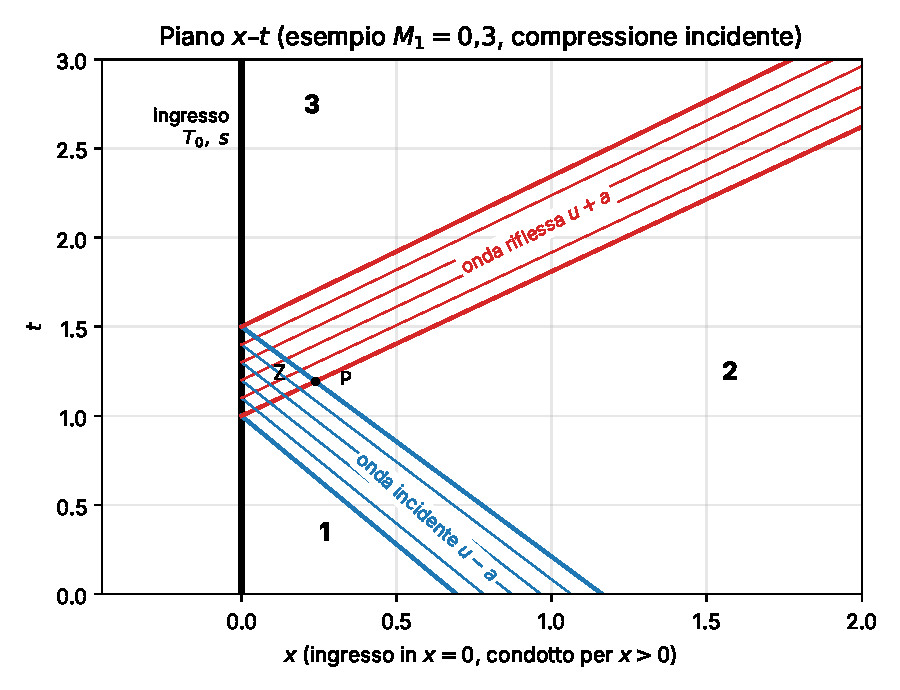
\includegraphics[width=0.68\textwidth]{xt.pdf}
  \caption{Piano $x$--$t$ vicino all'ingresso (esempio $M_1=0{,}3$, compressione incidente), con caratteristiche
  rettilinee: stati 1, 2, 3 e zona d'interazione Z.}
  \label{fig:xt}
\end{figure}
Nella fig.~\ref{fig:xt} l'incidente $\uma$ (blu) arriva all'ingresso fra $t=1$ e $t=1{,}5$; è una compressione, e
infatti le sue caratteristiche convergono. Ogni sua caratteristica genera nello stesso istante una $\upa$ della
riflessa (rosso), che si apre a ventaglio: è un'espansione. Le $\upa$ sono più veloci delle $\uma$ ($a+u>a-u$),
quindi più vicine all'orizzontale, e la riflessa occupa nello spazio un tratto più lungo dell'incidente: per
questo il suo gradiente è minore di quello dell'incidente. Le due onde si sovrappongono nel triangolo Z, chiuso dal
punto P.

\begin{figure}[H]
  \centering
  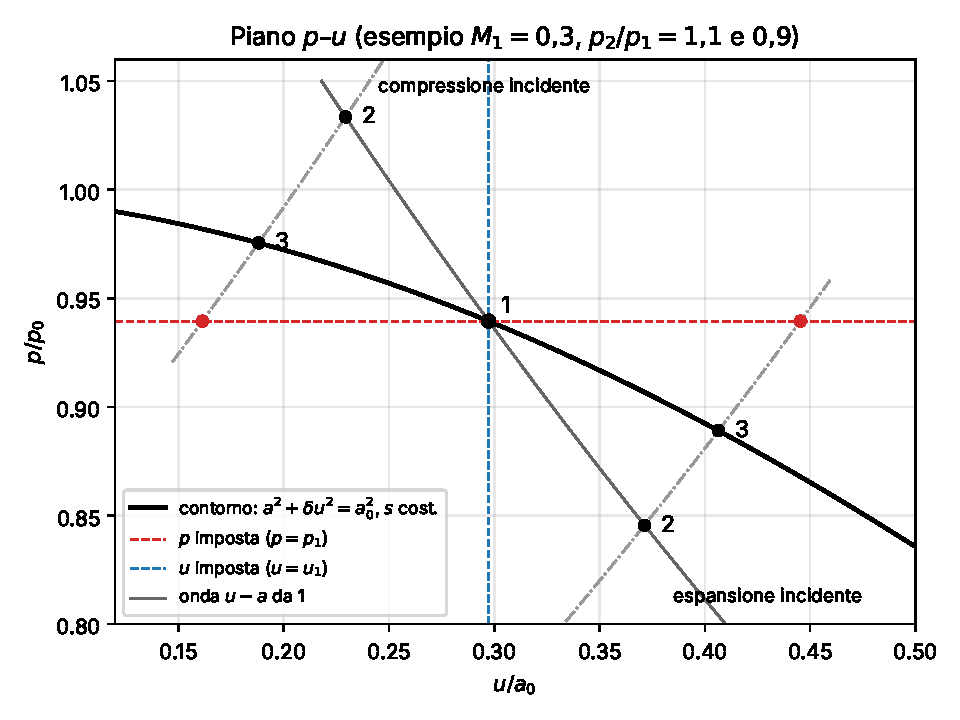
\includegraphics[width=0.72\textwidth]{pu.pdf}
  \caption{Piano $p$--$u$ (esempio $M_1=0{,}3$): curva del contorno $a^2+\delta u^2=a_0^2$ a $s$ costante e
  confronto con pressione e velocità imposte, per un'incidente di compressione ($p_2/p_1=1{,}1$) e di espansione
  ($0{,}9$).}
  \label{fig:pu}
\end{figure}
Nella fig.~\ref{fig:pu} lo stato 2 sta sulla curva dell'onda $\uma$ uscente da 1. Lo stato 3 è l'intersezione
della curva della riflessa $\upa$ uscente da 2 (tratto-punto) con la curva del contorno, che è la legge isentropica
$p=p_0(1-\delta u^2/a_0^2)^{\gamma/(\gamma-1)}$: poco inclinata, perché la sua pendenza è $dp/du=-\rho u$. Lo stato
3 cade dalla parte opposta di 2 rispetto a 1 in pressione: la riflessa ha natura opposta all'incidente. Cade fra
il punto a pressione imposta (rosso) e lo stato 2, più vicino al primo: a $M_1=0{,}3$ l'ingresso si comporta in
buona parte come un estremo aperto. Le pressioni coprono un intervallo stretto, quindi basta la scala lineare.

\begin{figure}[H]
  \centering
  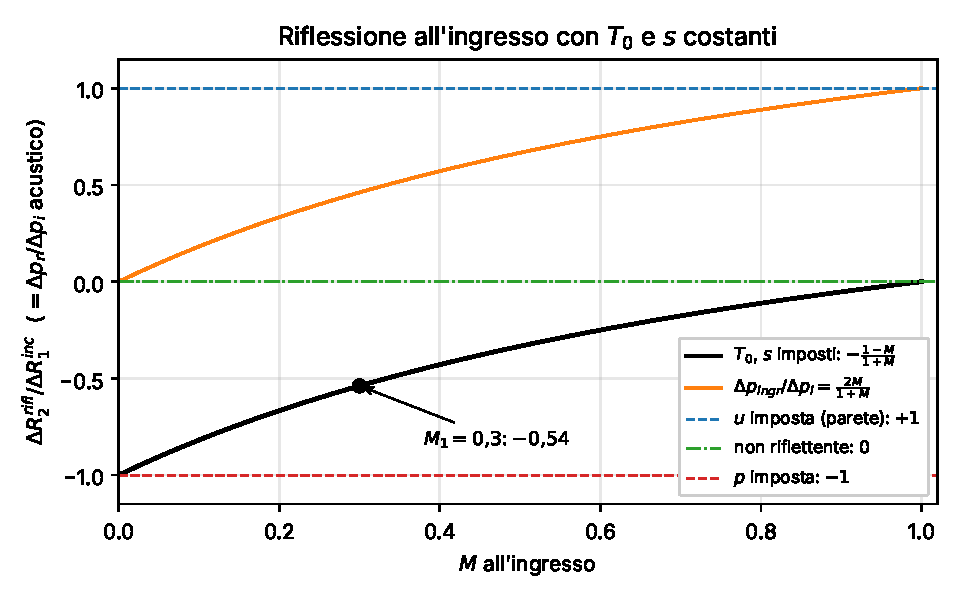
\includegraphics[width=0.72\textwidth]{coeff_riflessione.pdf}
  \caption{Coefficiente di riflessione all'ingresso e variazione di pressione nella sezione in funzione di $M$
  (aria), confrontati con velocità imposta, contorno non riflettente e pressione imposta.}
  \label{fig:C}
\end{figure}
La fig.~\ref{fig:C} riassume la risposta: il coefficiente sta fra $-1$ (pressione imposta, $M\to0$) e $0$ (non
riflettente, $M\to1$), sempre negativo. La curva arancione mostra quanto della perturbazione di pressione resta
nella sezione d'ingresso: poca a basso Mach, quasi tutta vicino a $M=1$.

%==============================================================================
\section{Discussione fisica}
\textbf{Che cosa rappresenta la condizione.} $T_0$ e $s$ costanti sono l'ingresso da un grande serbatoio o
dall'ambiente: il gas accelera dal ristagno alla sezione d'ingresso senza perdite e in modo quasi stazionario, quindi
lì valgono istante per istante $h_0$ e $p_0$ del serbatoio. Nel tempo il legame è Bernoulli, $dp=-\rho u\,du$: la
pressione può cambiare solo se cambia la velocità, e a basso Mach cambia poco.

\textbf{Perché la natura opposta.} Al contorno sinistro una relazione lineare $\Delta u=k\,\Delta a$ dà
\[
  \frac{\Delta\Rd}{\Delta\Ru}=\frac{1+\delta k}{1-\delta k}.
\]
Con velocità imposta ($k=0$) il coefficiente è $+1$; con pressione imposta ($k\to\infty$) è $-1$; il contorno non
riflettente ($\Rd$ costante) richiede $k=-1/\delta$. Qui $\Delta a=-\delta M\,\Delta u$, cioè $k=-1/(\delta M)$, e
$|k|>1/\delta$ per ogni $M<1$: la riflessione ha sempre
natura opposta, fra l'estremo aperto e il contorno non riflettente. Per l'uscita a Mach imposto (B70-E02) succedeva
il contrario, con riflessione della stessa natura.

\textbf{La portata.} Da $\dot m_t/\dot m=(1-M^2)\,u_t/u$, una compressione che arriva dall'interno riduce la
portata che entra e un'espansione la aumenta: il serbatoio ``sente'' il condotto. Con $M\to1$ la portata non può
più cambiare, perché ha raggiunto il massimo fissato da $p_0$ e $T_0$.

\textbf{Confronto con altri ingressi.} Con portata ed entalpia totale imposte (B68-E02) l'entropia del gas che
entra non è fissata e dall'ingresso parte anche un'onda di entropia. Qui l'omoentropia la esclude ($Z=0$), e
l'unica onda entrante è la $\upa$.

\textbf{Limiti di validità.} Le formule valgono finché il gas entra ed è subsonico. Nell'esempio una compressione con
$p_2/p_1\approx1{,}27$ annulla la velocità all'ingresso: oltre, il gas rifluisce nel serbatoio, l'ingresso diventa
un'uscita con una sola caratteristica entrante, e la condizione diventa $p=p_0$; imporre ancora $T_0$ sarebbe una
sovraspecificazione. Un'espansione con $p_2/p_1\approx0{,}47$ porta invece l'ingresso a $M=1$. A quel punto la
$\uma$ è verticale: lo stato resta quello critico, $a=a_0\sqrt{2/(\gamma+1)}$, e il resto dell'espansione non
raggiunge più l'ingresso, che rimane sonico.

\end{document}
